\documentclass[10pt,twocolumn,letterpaper]{article}

\usepackage{acvs}
\usepackage{times}
\usepackage{epsfig}
\usepackage{graphicx}
\usepackage{amsmath}
\usepackage{amssymb}

% Include other packages here, before hyperref.
\usepackage{dsfont}

% If you comment hyperref and then uncomment it, you should delete
% egpaper.aux before re-running latex.  (Or just hit 'q' on the first latex
% run, let it finish, and you should be clear).
\usepackage[pagebackref=true,breaklinks=true,letterpaper=true,colorlinks,bookmarks=false]{hyperref}

\iccvfinalcopy % *** Uncomment this line for the final submission

\def\iccvPaperID{} % *** Enter the Paper ID here
\def\httilde{\mbox{\tt\raisebox{-.5ex}{\symbol{126}}}}

% Pages are numbered in submission mode, and unnumbered in camera-ready
\ificcvfinal\pagestyle{empty}\fi

\begin{document}

%%%%%%%%% TITLE - PLEASE UPDATE
\title{RePaint: Inpainting using Denoising Diffusion Probabilistic Models~\cite{repaint} \\ {\rm {\normalsize Minji Kim (minji@snu.ac.kr; 2020-28702), Dept. of Electrical and Computer Engineering, Seoul National University}}}   % **** Enter the paper title and student information here

\maketitle
\thispagestyle{empty}

%%%%%%%%% BODY TEXT - ENTER YOUR RESPONSE BELOW

%%%%%%%%%%%%%%%%%
%%%%%%%%%%%%%%%%%
\section{Introduction}
Inpainting is a process of reconstructing damaged, deteriorated, or missing parts of images or videos.
Early approaches include searches for the most similar patches from the untacted pixels of the image itself, and then directly pastes the patches on the missing parts.
On the other hand, there were GAN-based approaches such as Context Encoder, GLCIC.
The problem of previous inpainting models is that 1) they are not generalizable to unseen mask types, and 2) training with pixel-wise and perceptual loss often leads to naive textural extensions instead of semantically meaningful generation.
To cope with this limitation, the authors propose \textbf{RePaint}, which conditions the generation process by sampling from the given pixels during the reverse diffusion iterations, instead of learning a mask-conditional generative model.
As shown in Fig.~\ref{fig:teaser}, Denoising Diffusion Probabilistic Models (DDPM) is used for inpainting.
The process is conditioned on the masked input, and it starts from a random Gaussian noise sample, and than it is iteratively denoised until a high-quality output is generated.
As this process is stochastic, multiple diverse outputs can be obtained.



%%%%%%%%%%%%%%%%%
%%%%%%%%%%%%%%%%%
\section{RePaint}

\subsection{Overview}
The overview of Repaint is shown in Fig.~\ref{fig:overview}.
RePaint modifies the standard denoising process in order to condition on the given image content.
In each step, it samples the known region from the input and the inpainted part from the DDPM output.
Specifically, given a ground truth image $x$, the unknown pixels $m \odot x$ and the known pixels $(1-m) \odot x$, the known regions in diffusion step $t$, $(1-m) \odot x_t$, could be consistently altered.
Thus, in each reverse step, $x_{t-1}$ could be obtained by using following equations:
%
\begin{equation}
    x^{known}_{t-1} \sim \mathcal{N}(\sqrt{\bar{\alpha}_t}x_0, (1-\bar{\alpha}_t)\mathbf{I}),
\end{equation}
\begin{equation}
    x^{unknown}_{t-1} \sim \mathcal{N}(\mu_\theta(x_t, t), \Sigma_\theta(x_t, t)),
\end{equation}
\begin{equation}
    x_{t-1} = m \odot x^{known}_{t-1} + (1-m) \odot x^{unknown}_{t-1}.
\end{equation}
%
Thus, $x^{known}_{t-1}$ is sampled using the known pixels in the given image $m \odot x_0$, and $x^{unknown}_{t-1}$ is sampled from the model, given the previous iteration $x_t$ is given.
Finally, the new sample $x_{t-1}$ is combined using the mask.

\subsection{Resampling}
Using above algorithm, the inpainted region might mismatches the neighboring regions semantically, because the sampling of the known pixels is performed without considering the generated parts of the image.
The model needs more time to harmonize the conditional information $x^{known}_{t-1}$ with the generated information $x^{unknown}_{t-1}$ in one step before going to the next denoising step.
Thus, they use the property of DDPM which aims at producing consistent structure, and resample by diffusing the output $x_{t-1}$ back to $x_t$.


%%%%%%%%%%%%%%%%%
%%%%%%%%%%%%%%%%%
\section{Conclusion}

This paper has proposed mask-agnostic inpainting model.
DDPM is applied during inpainting, while the training is stabilized with resampling strategy.
The limitation of this paper is that RePaint is significantly slower than other approaches such as GAN-based or Autoregressive-based methods.


\begin{figure}[t]
    \includegraphics[width=\linewidth]{assets/teaser.png}
    \caption{\label{fig:teaser}DDPM for inpainting.}
\end{figure}

\begin{figure}[t]
    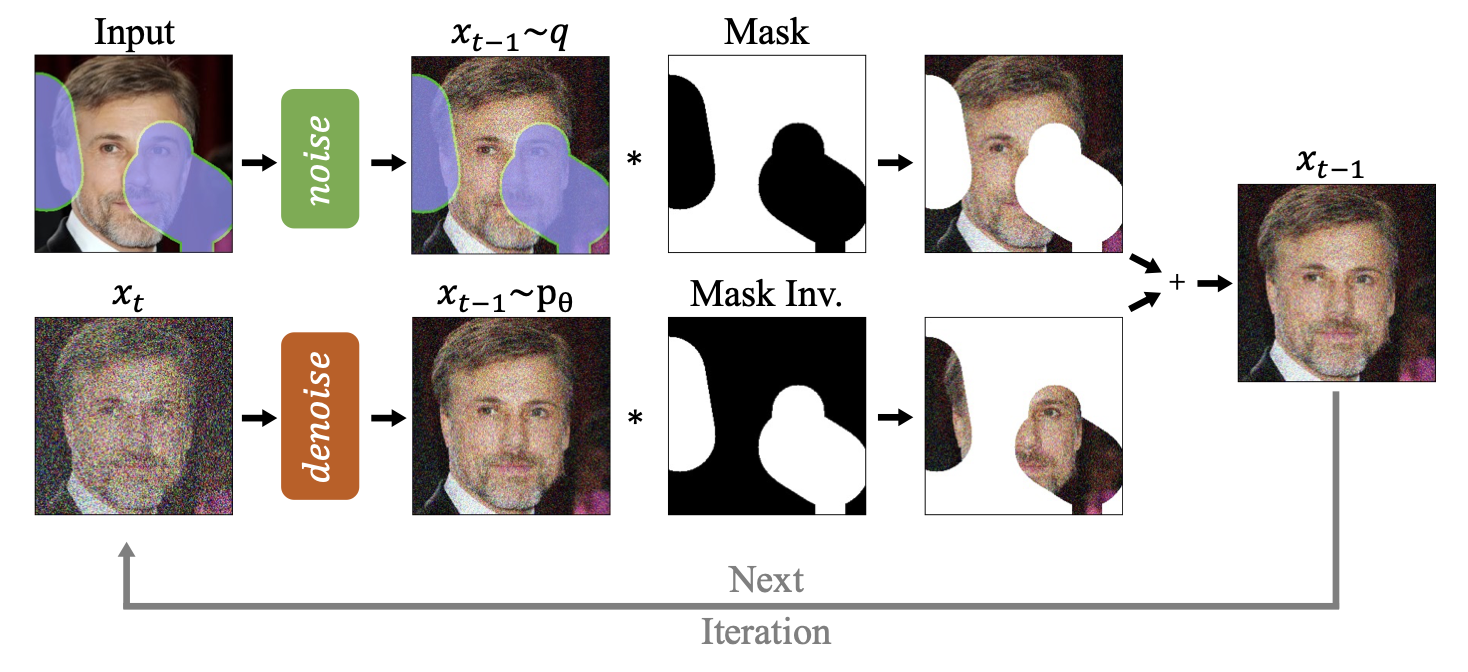
\includegraphics[width=\linewidth]{assets/overview.png}
    \caption{\label{fig:overview}Overview of Repaint.}
\end{figure}




{\small
\bibliographystyle{ieee}
\bibliography{egbib}
}

\end{document}
